\section{Introduction}

% Motivation
The University of Melbourne's cold-atom electron source aims to be able to create high-brightness, high-coherence electron bunches for use in coherent electron diffractive imaging. Imaging of nanoscale objects such as biological molecules\cite{dwyer_femtosecond_2006, williamson_clocking_1997} and defects in solid-state devices\cite{siwick_atomic-level_2003} by ultrafast, single-shot electron diffractive imaging would provide important information about structure and dynamic processes of nanoscale objects.

Membrane proteins, for example, are very important for some reason \emph{(ASK VIVIEN get some references)}. Determining the structure of these molecules is a key step in understanding their chemical and biological function. The importance of knowing the atomic structure of biomolecules is exemplified by the enormous progress made in various fields of biology once the double-helical structure of DNA was determined from x-ray images in 1953\cite{watson_molecular_1953}. Once a protein's structure and function are known then it becomes possible to design drugs\cite{pinto_influenza_1992} where needed and to more fully understand how the protein behaves in its biological system.

In order to determine the structure of these biological molecules atomic, sub-nanometre imaging resolution is required. A number of techniques are available for determining these structures \cite{nettleship_methods_2008, svergun_small-angle_2003, opella_structure_2004} however the most successful to date has been x-ray crystallography \cite{kendrew_three-dimensional_1958, uson_advances_1999}. Unfortunately the process of crystallising these membrane proteins is difficult and to date relatively few have been crystallised \cite{geerlof_impact_2006}.

New imaging techniques and light sources such as x-ray free electron lasers and  ultrafast single-shot diffraction have been driven by the goal of overcoming the limitations of x-ray crystallography. Ultrafast single-shot diffraction imaging also has the potential to determine dynamic structure of biological molecules. The Melbourne cold-atom electron source is aims to produce bright, coherent bunches of electrons for use in diffractive imaging.

\subsection{Ultrafast, single-shot, coherent diffractive imaging with electrons}
X-ray diffraction from crystals was first observed a century ago\cite{bragg_x-rays_1912} and resulted in a Nobel prize being awarded to William Bragg and his son. Since then \gls{cdi} has been performed on a myriad of different samples with coherent beams of x-rays and electrons.

Electrons have a shorter wavelength than x-rays thus allowing a higher limit on the attainable resolution for \gls{cdi}. [REFERENCE would be nice] 

\subsubsection{Single-shot diffractive imaging}
Single-shot diffractive imaging with an x-ray source of sufficient brightness should be able to produce a diffraction pattern from scattered x-rays from a single molecule before the molecule is destroyed by the Coulomb explosion which follows photoionisation within the molecule\cite{henderson_potential_1995, neutze_potential_2000}. Single-shot imaging aims to avoid the need for crystallisation with x-ray imaging since with a sufficiently bright source should allow imaging of any molecule.

With femtosecond timescale single-shot imaging it becomes possible to observe such things as molecular vibration and dynamic chemical processes\cite{zewail_4d_2006} with the sophisticated imaging techniques currently in development it will become possible to create ``molecular movies''\cite{dwyer_femtosecond_2006} of these processes.

\subsection{Melbourne cold-atom electron source}
The University of Melbourne's cold-atom electron source project aims to produce an electron source for coherent diffractive imaging. If bright, coherent, femtosecond long bunches of electrons can be produced then \gls{cdi} can be performed on a range of structures.

The cold-atom electron source operates by first illuminating laser-cooled rubidium atoms with a resonant 780 nm excitation laser followed by a 5 ns 480 nm ionisation laser pulse. The electrons are then accelerated in a uniform electric field and guided and focused onto the target.

[CHANGE THE FIGURE SO IT DOESN'T HAVE THE DIPOLE TRAP]
\begin{figure}[h]
	\centering
	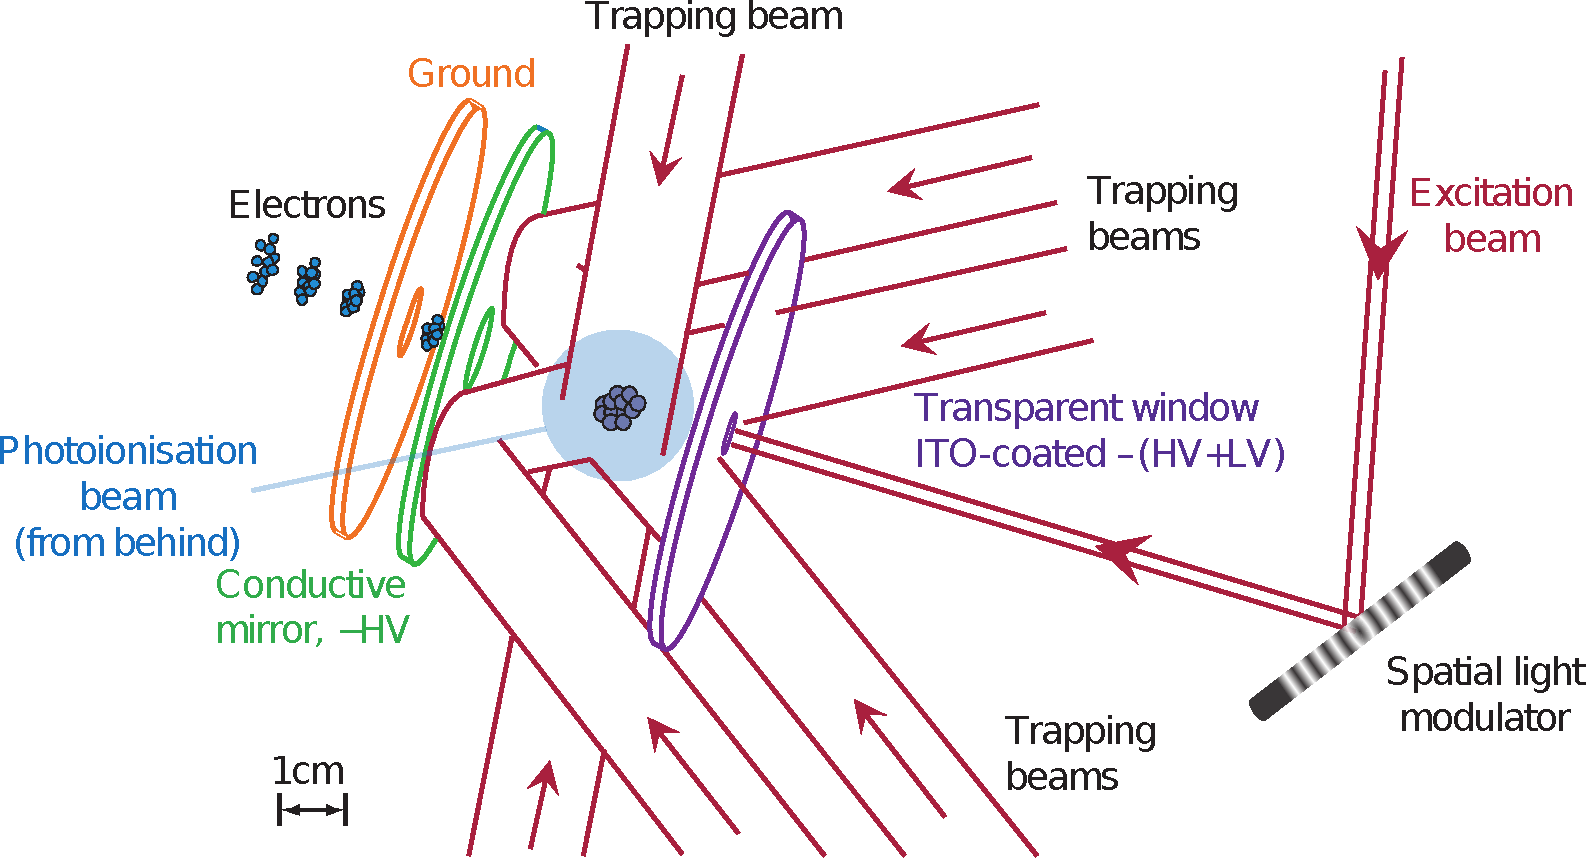
\includegraphics[scale=0.32]{figs/MOT.pdf}
	\caption[Title]{Quasi mirror MOT with \gls{odt}}
	\label{figs/MOT.pdf}
\end{figure}

When extracting the ionised electrons from the atom cloud it is necessary to turn off the magnetic trapping fields [AND THE ZEEMAN SLOWER?] in order to prevent magnetic distortions of the electron bunches' paths. This means that just before electron extraction the cloud is no longer trapped and is beginning to expand. The use of trapping mechanisms that do not interfere with the electron bunches, such as an \gls{odt}, will help prevent this expansion and thus stabilise the initial position of the electron bunches which tend to drift at present due to dispersal of current, and hence magnetic field, in the magnetic coils and their power supplies.

Using an \gls{odt} in this system will also allow an increase in the brightness and coherence of the source due to higher atom cloud densities during the ionisation process.

\subsubsection{Brightness}
Brightness is important in single-shot \gls{cdi} due to the need to maximise the scattered signal and thus ensure sufficient sampling of the specimen within the exposure time.

For the cold-atom source the transverse brightness at the source is given by\cite{reiser_theory_2008}
\begin{equation}
B_\perp = \frac{I_p m_e c^2}{4 \pi^2 \sigma_x \sigma_y k_B T},
\end{equation}
where $\sigma$ is the root mean squared source size and $I_p$ is the peak electron current.

A pulse of electron's brightness can be increased by a reduction in the length of the bunches, by increasing the density of the bunches or by increasing the number of electrons in the bunch. A short bunch is necessary for ultrafast electron diffraction.

The use of an \gls{odt} will allow an increase of the atom-cloud density which will in turn result in an increase of the electron bunch density.

\subsubsection{Coherence}
Unsurprisingly coherence is an important factor in \gls{cdi} since this technique relies on the interference of the diffracted waves. The transverse coherence length of a imaging beam must be approximately twice the width of the object being imaged\cite{spence_coherence_2004}.

For a quasi-homogeneous source\cite{nugent_coherent_2009}, the transverse coherence length $L_c$ can be related to the transverse momentum spread, and hence the temperature, through\cite{van_oudheusden_electron_2007}
\begin{equation}
L_c = \hbar/\sqrt{m_e k_B T}.
\end{equation}

The transverse coherence is determined solely from the temperature of the electrons which is proportional to the temperature of the electron source and the ionisation energy.

The coherence of our electron bunches will be increase with the correct use of an \gls{odt} since the trap will serve to reduce the temperature of the atom cloud, and hence the electron bunches.


